\chapter{Quality Assurance} \label{cha:qa}
	This chapter explains and describes various quality assurance techniques 
	that were used during the project, to allow us to deliver a product of 
	good quality (regarding both code quality and gameplay quality). It also
	talks a bit about Microsoft Visual Studio first, our IDE of choice for
	this project, considering that some QA tools are not available for
	MonoDevelop, the standard IDE packaged with Unity.
	
	\section{IDE used for programming} \label{sec:ide}
		The IDE used for programming was Microsoft Visual Studio. Unity has an IDE
		of its own available for programming in C\#, which is called MonoDevelop.
		However, the MonoDevelop IDE is really lacking in functionality. It has no
		support for the plugins that we use to check our code. Furthermore, the use
		of MonoDevelop enforces a code style that is incompatible with the style 
		guidelines used by StyleCop (see \ref{sec:codestyle}), 
	
	\section{Testing} \label{sec:testing}
		There are two main types of testing done during the project. These are
		unit testing and integration testing. Unity has no native support for
		running unit\slash integration tests that have been written, but there is 
		a toolkit available for free on the Asset Store, called Unity Test Tools, 
		that does have this support. The extension is developed by the Unity team, 
		and can be found on the Unity Asset Store: 
		\url{https://www.assetstore.unity3d.com/en/#!/content/13802}.
		Using this extension, a new menu bar item, called "Unity Test Tools"
		will appear in the main Unity editor. Clicking on this item creates a drop
		down menu with different options, the most important one being the unit test
		runner.
		
		\subsection{C\# Unit Tests} \label{ssec:csharpunittests)}
			Unit tests are written using the NUnit unit testing framework for 
			C\#. NUnit is a test framework which was ported from the Java test 
			framework JUnit, and was created to bring xUnit testing to all .NET 
			languages. Using this framework is also really easy, and a tutorial 
			on how to write unit tests using NUnit can be found using Google. 
			Using Unity Test Tools, all unit tests in the project are listed 
			once one clicks on the subitem "Unit Test Runner". The tests are 
			listed in a new window, and one can run all unit tests by clicking 
			on the "Run All" button at the top. The menu then shows what unit 
			tests have passed or failed, and clicking on a unit test shows what 
			went wrong. A unit testing overview can be seen in \ref{fig:unitytesttools}.
			The UnityTest testing class seen in the overview also displays
			the different statuses of tests in the NUnit framework (passing,
			failing, inconclusive, not executed, and culture specific).
			
			\begin{figure}[!ht]
				\centering
				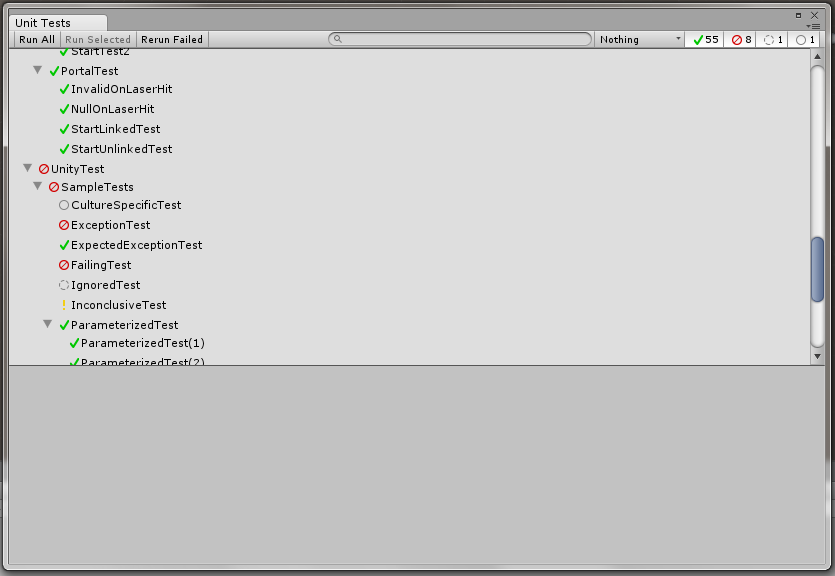
\includegraphics[width=\textwidth]{UnityTestTools}
				\caption{The Unity Test Tools unit testing screen.}
				\label{fig:unitytesttools}
			\end{figure}
			
		\subsection{C++ Unit Tests} \label{ssec:cplusplusunittests}
			...
		
		\subsection{Integration Tests} \label{ssec:integrationtests}
			Integration tests are not done via a formalized test procedure, but 
			rather by creating simple scenes and observing that the subjects of 
			the test work as they should when they are placed in an actual 
			scene. It is also a lot harder to run these tests in a standardized 
			way most of the time. 
		
		\subsection{Code coverage} \label{ssec:codecoverage}
			Code coverage is a metric that can be used to determine how thorough
			the written code has been tested. There are several free software
			packages available on the Internet that allow for generating code
			coverage reports of NUnit test suites, such as NCover or PartCover.
			These, however, are hard to use when combined with unit tests in
			Unity. The reason behind this is that, to run the unit tests for
			the game, the Unity Test Tools functionality has to be used (as most
			tests use instantiation of gameplay objects, something that can
			only happen in Unity). This functionality has no way of integrating
			the NCover or PartCover software packages. It is possible to integrate
			these with Microsoft Visual Studio, however it is impossible to run
			the unit tests from that IDE. As such, we had to manually check
			if the tests tested all possible branches of the code.
			
	\section{Code Style} \label{sec:codestyle}
		We decided to stick to the code style guidelines defined by StyleCop and 
		FxCop, two utilities developed by Microsoft. These utilities check for 
		common programming and code style errors in projects so that these can 
		easily be identified and fixed. 
		
		During the project, we kept the source code style checked by periodically
		dedicating time solely for checking code style and performing code 
		maintenance. This also included writing or improving unit tests and 
		refactoring classes and methods with a relatively high complexity or other 
		issues as indicated by StyleCop and FxCop.
		
	\section{SonarQube} \label{sec:sonarqube}
		For getting a clear overview of the source code quality of the project, as 
		well as the issues indicated by FxCop and StyleCop (see section 
		\ref{sec:codestyle}), we made use of a SonarQube server, hosted on one of 
		our development machines. SonarQube keeps track of issues indicated by 
		the abovementioned tools, and performs various code metrics, like cyclomatic 
		complexity and dependency cycles. Using SonarQube enabled us to spot 
		problematic classes and methods and allowed us to improve the overall 
		structure of the source code of the project. An example of a SonarQube
		overview can be seen in figure \ref{fig:sonarqube}
		
		\begin{figure}[!ht]
			\centering
			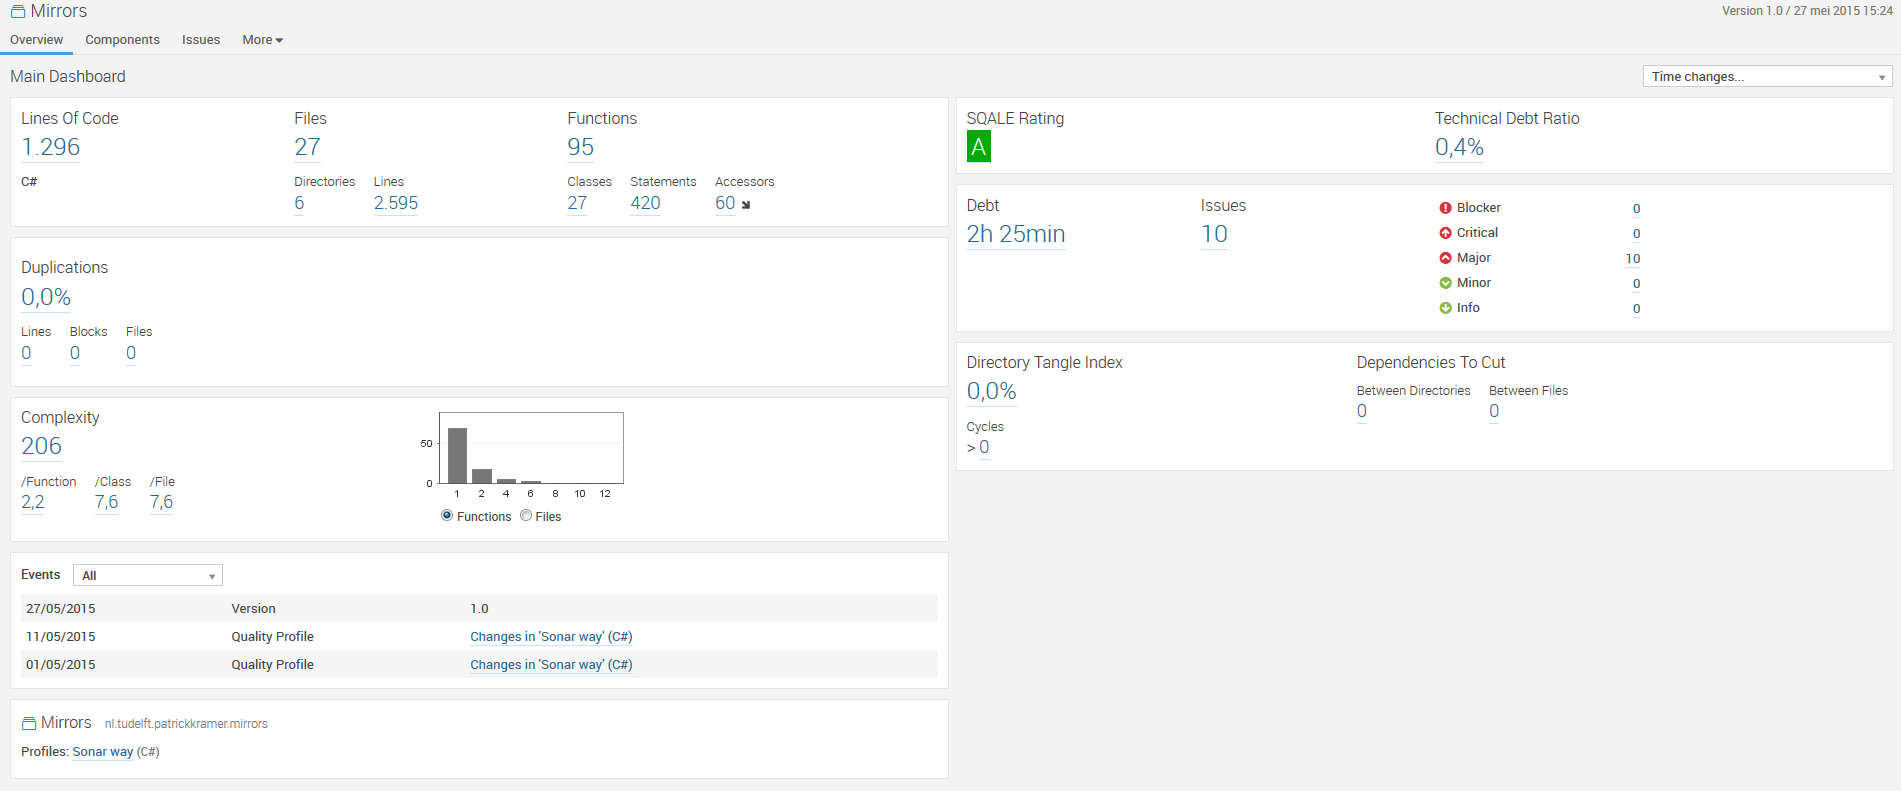
\includegraphics[width=\textwidth]{SonarQube}
			\caption{A SonarQube overview.}
			\label{fig:sonarqube}
		\end{figure}
		
		An issue with SonarQube is that, while it has free options for analyzing
		C\# code, it has none of these free options for analyzing C/C++ code,
		because of the preprocessing that can happen in C or C++ (as explained
		in their blog on \url{http://www.sonarqube.org/ccobjective-c-dark-past-bright-future/}).
		For this reason, it is very hard to analyze the C++ code that we use for the
		OpenCV server.
		
	\section{SIG Evaluation} \label{sec:sigevaluation}
		SIG is an acronym which stands for the Software Improvement Group,
		which is a company that is based in Amsterdam. The company does code
		analysis to evaluate code quality on a scale from one to five stars,
		and it does so according to the ISO/IEC 25010 model. Code score is 
		based on the maintainability of the code. During the project, there 
		are two opportunities to deliver the code that we have written to
		SIG. The first opportunity is at the end of May, and the second is
		halfway through June. The first opportunity is used as a midterm
		quality feedback session, for us to get feedback about how good
		the code is written and what can be done better. The second opportunity
		is then intended to hand in the improved code, and for us to then
		get feedback on how well the code has been improved. The improvements
		in the code also have a weight in the final result for the project.
		
	\section{Demo's and playtesting sessions} \label{sec:demos}
		%TODO Write about the demo with the client.
		...
